\section{Strongly Coupled Dark Matter}\label{sec:darkqcd}

\subsection{SVJ Models}\label{subsec:models}

Dark QCD models include numerous parameters, with current searches focusing on those most immediately observable:
the mediator mass \mZprime or \mbifun, the dark hadron mass scale \mdark, and the invisible fraction \rinv.
The latter is the most novel parameter of the model, corresponding to the fraction of dark hadrons that are stable and invisible (DM candidates).
However, it is an effective parameter, summarizing the impacts of various accidental symmetries and conserved quantum numbers.
Many other dark sector parameters can impact the collider final state, including the cutoff scale \Lamdark, the dark quark mass \mqdark, the number of dark colors \Ncdark, and the number of dark flavors \Nfdark.
The details of the mediator connecting the SM and dark sector, such as its couplings, can affect the decays of unstable dark hadrons.
In addition, because low-energy QCD bound state formation via showering and hadronization is non-perturbative, it must be simulated using phenomenological models,
with parameters that are tuned to measurements of SM QCD and may not be identical in dark QCD.

The models currently investigated in CMS searches are based on Refs.~\cite{Cohen:2015toa,Cohen:2017pzm}, along with contributions from the PI
regarding the relationship between \mdark and \Lamdark, as well as the modeling of \rinv~\cite{Albouy:2022cin}.
These models choose $\Ncdark=2$ and $\Nfdark=2$, which leads to similarities in baryon and meson states that may not be modeled correctly,
given the lack of a confining $SU(2)$ force in the SM.
Here, we propose a more comprehensive assessment of the interplay between \Nfdark, \Lamdark, \mdark, and \mqdark (among other parameters),
focusing on the $\Ncdark=3$ case, for which lessons from the SM, especially from lattice QCD, can be more easily reused.
This follows directly from the Snowmass effort in Ref.~\cite{Albouy:2022cin}, which presented a few benchmarks of more realistic dark QCD models.
The result will be a complete set of benchmarks covering the entire range of \rinv values from 0 to 1,
reflecting new understanding about degeneracies in the model space and any nontrivial correlations between \rinv and observables such as jet substructure.
This new set of benchmarks can guide the Run 3 search strategy to ensure the entire known phase space is covered
and can serve to unify the efforts of different experimental collaborations, which currently study different models.

\subsection{SVJ Searches}\label{subsec:searches}

\begin{figure}[htb!]
\centering
\twofigeqh{figures/comp_limit_dijet_new_svj_monojet_2d.pdf}{{figures/comp_gq_dijet_orig_svj_monojet_rinv0.3}.pdf}
\caption{Excluded regions of the \mZprime-\rinv plane (left) and limits on \gq (right) from the SVJ search, dijet search, and monojet search.
}
\label{fig:svjexcl}
\end{figure}

\begin{figure}[htb!]
\centering
\twofigeqh{figures/axol1tl_score_schan.pdf}{figures/axol1tl_score_tchan2.pdf}
\caption{Score distributions from anomaly triggers on SVJ processes. (PLACEHOLDER)}
\label{fig:svjanomaly}
\end{figure}

\begin{figure}[htb!]
\centering
\twofigeqh{figures/rocScoreSigP2DQCD_rinv.pdf}{figures/WNAE_performance_from_SVJ_t_channel_status_update_2024_02_06-2.pdf}
\caption{The performance of the latest SVJ taggers: supervised ParticleNet (left) and unsupervised Wasserstein normalized autoencoder (right).
A score of 1.0 would indicate perfect discrimination between signal and background jets.}
\label{fig:svjtaggers}
\end{figure}

% centered, fixed-width column type
\newcolumntype{C}[1]{w{c}{#1}}
\newlength\searchlen
\setlength\searchlen{1cm}
\newlength\searchlena
\setlength\searchlena{2\searchlen}
\newlength\searchlenb
\setlength\searchlenb{3\searchlen}
\newlength\searchlenc
\setlength\searchlenc{6\searchlen}

\begin{table}[!hbtp]
\vspace{\myfigurespacing}
\centering
\begin{tabular}{c|*{6}{C{\searchlen}}}
\hline
\multirow{2}{*}{Mediator} & \multicolumn{6}{C{\searchlenc}}{Mass range} \\
& \multicolumn{2}{C{\searchlena}}{Low} & \multicolumn{2}{C{\searchlena}}{Medium} & \multicolumn{2}{C{\searchlena}}{High} \\
\hline
\PZprime & \multicolumn{2}{C{\searchlena}}{\cellcolor{yellow!50}\makecell{standard\\(boosted)}} & \multicolumn{2}{C{\searchlena}}{\cellcolor{magenta!50}\makecell{scouting\\\vphantom{(boosted)}}} & \multicolumn{2}{C{\searchlena}}{\cellcolor{orange!50}\makecell{standard\\\vphantom{(boosted)}}} \\
\hline
\Pbifun & \multicolumn{3}{C{\searchlenb}}{\cellcolor{orange!50}\makecell{standard\\\vphantom{(boosted)}}} & \multicolumn{3}{C{\searchlenb}}{\cellcolor{magenta!50}\makecell{scouting\\\vphantom{(boosted)}}} \\
\hline
\end{tabular}
\vspace{\myfigureskip}
\caption{A summary of the conventional trigger options to target different mediators and mass ranges for SVJ production.}
\label{tab:conventional}
\end{table}

% todo: add plot showing discovery significance for Run 2 vs Run 3, taking into account sqrt(s), lumi

\begin{figure}[htb!]
\centering
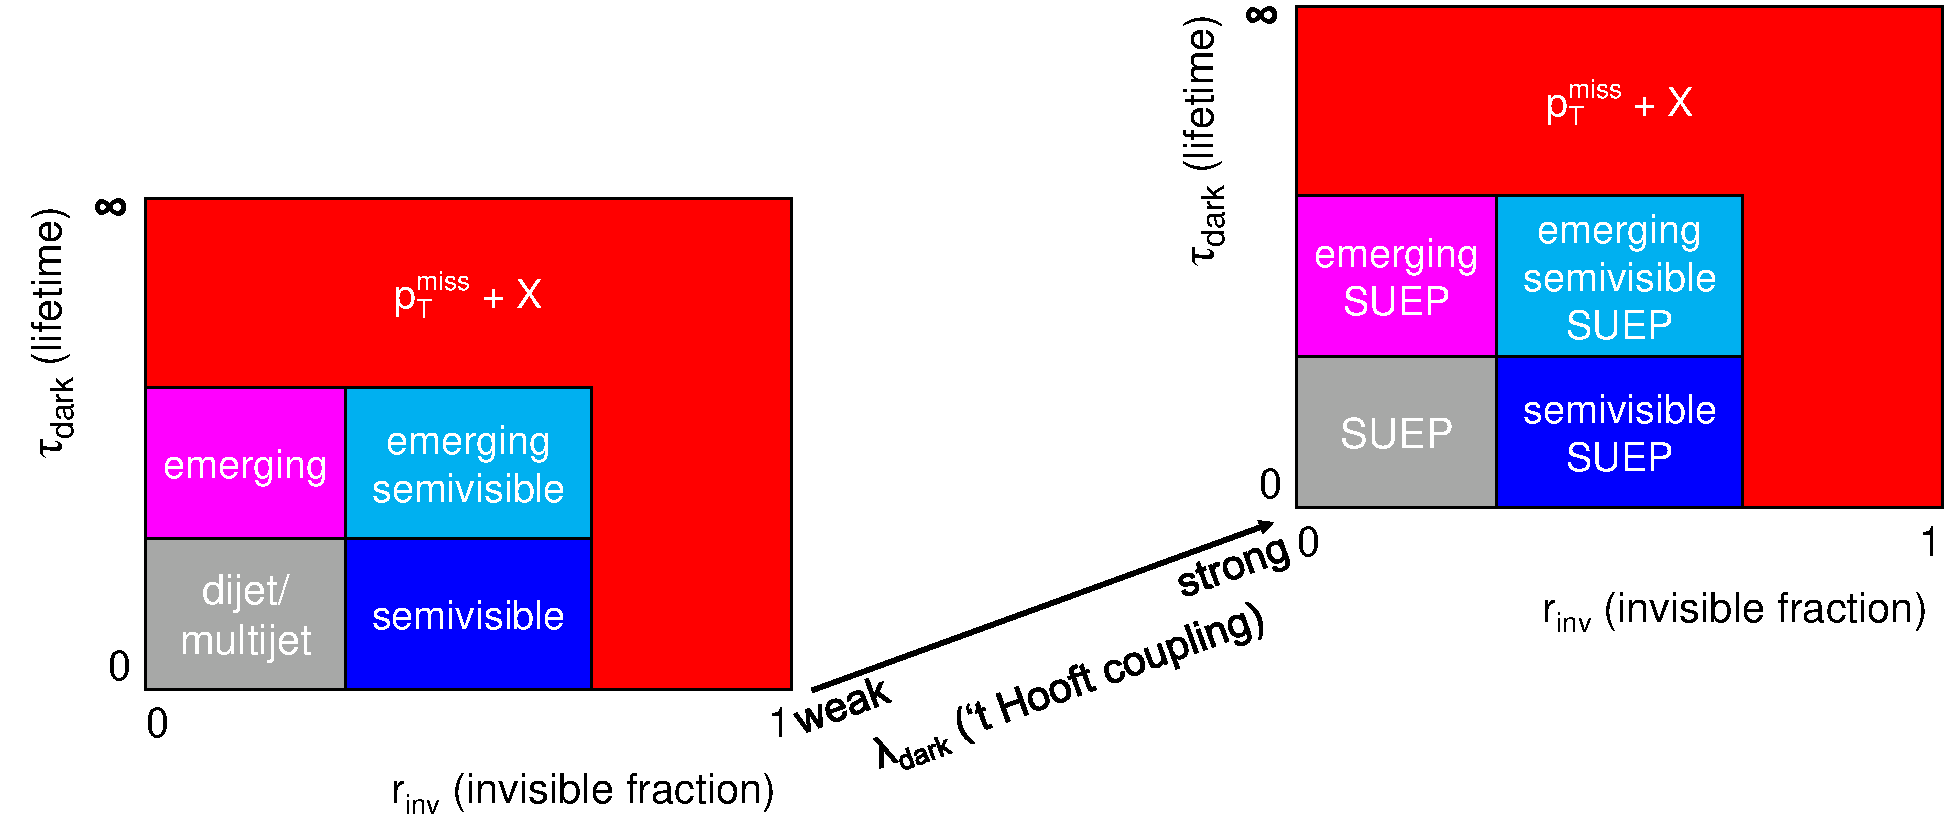
\includegraphics[width=0.95\myfigurewidth]{figures/svj_acceptance_diagram_v7.pdf}
\caption{A diagram illustrating the phenomena and search strategies with maximal acceptance for different combinations of dark QCD parameters.}
\label{fig:svjacc}
\end{figure}
